\section{Evaluation}
\label{sec:eval}

\subsection{Resource Utilization}
For evaluation of the resource utilization of the different implementations, the min-heap and tagged up/down sorted were synthesized with various different queue sizes until the required resources exceeded the resources available in the FPGA. The results were then compared with the published results of the state-of-the-art implementations. After performing these steps, it was clear that the resources in contention were the look-up tables (LUTs), flip-flops (sometimes known as slice registers) and block RAMs(BRAMs). Since these implementations generally do not need to interface with external devices, usage of only these resources is expected, as the modules are only operating in the FPGA. In addition, since these are not digital signal processing applications, but are highly combinatorial and memory-intensive, high usage of LUTs and BRAMs is also expected. However, it should be noted that the min-heap and tagged up/down sorter priority queues do not use any BRAM resources, as they only store the priorities with no associated data. Since the other queue implementations do store extra data, they make us of the BRAMs, so BRAM utilization is not analysed.

\begin{figure}[t!]
	\centering
	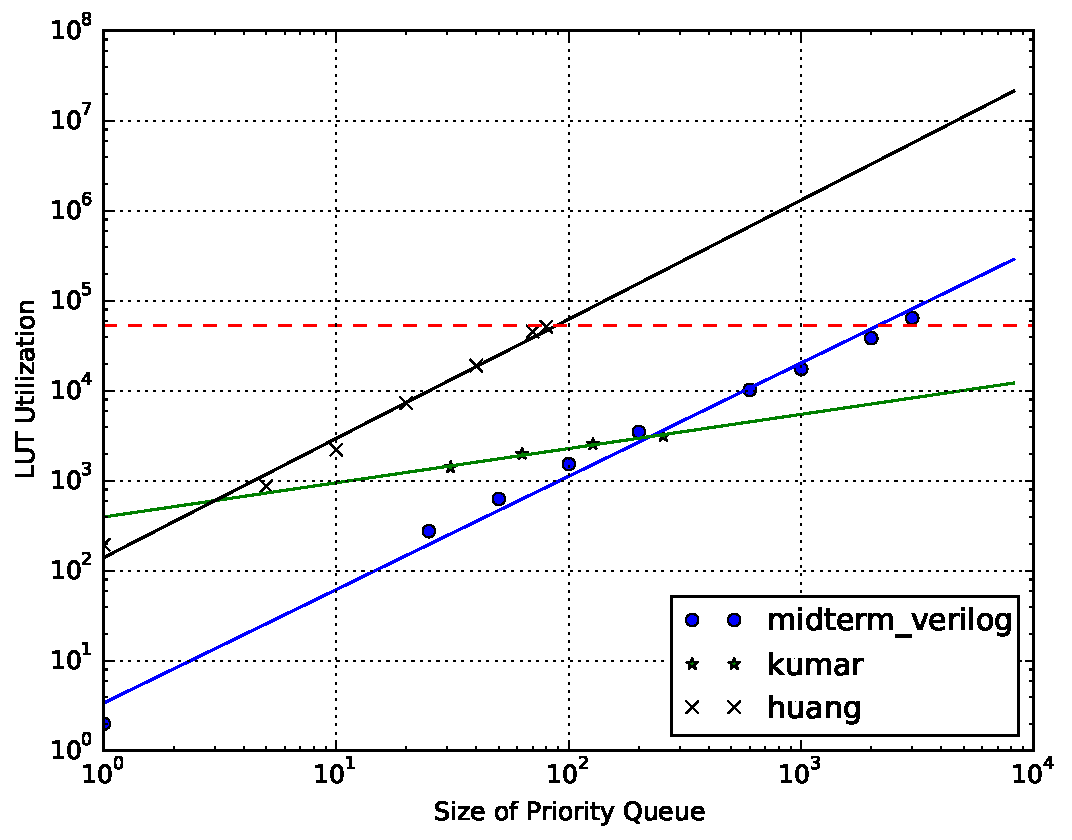
\includegraphics[width=\columnwidth]{data/lut_utilization.pdf}
	\caption{LUT Utilization}
	\label{fig:luts}
\end{figure}

\begin{figure}[t!]
	\centering
	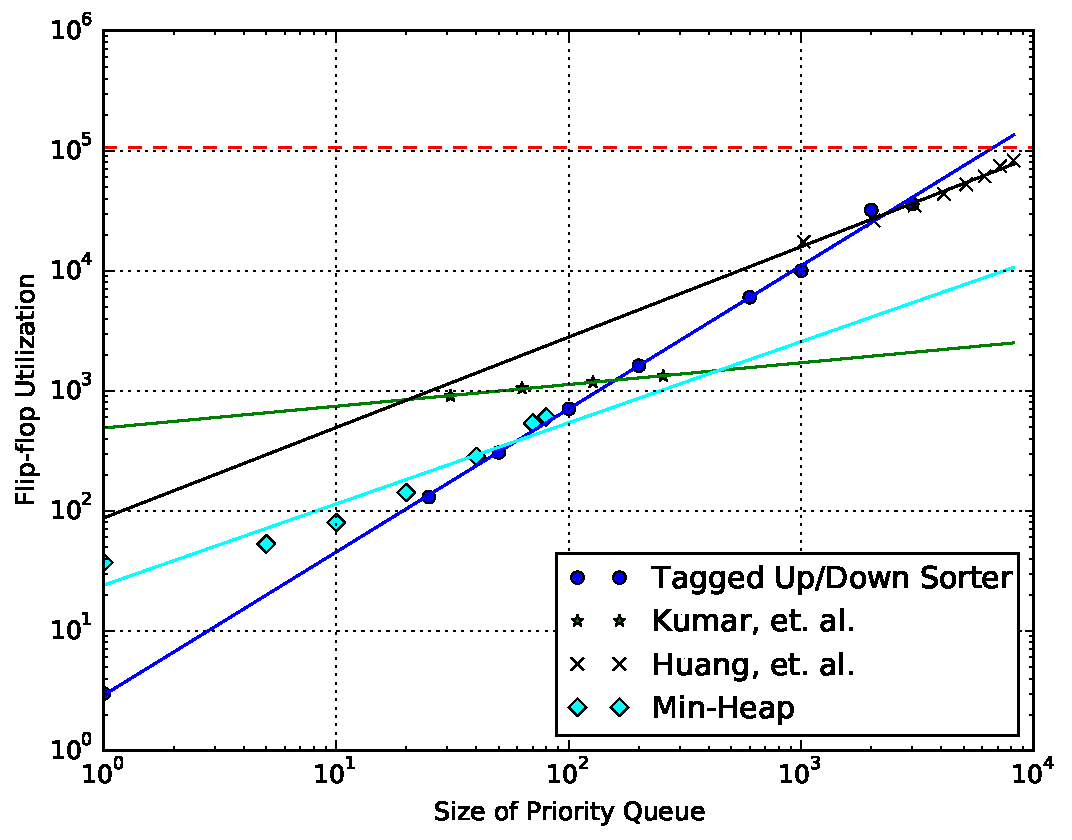
\includegraphics[width=\columnwidth]{data/ff_utilization.pdf}
	\caption{Flip-flop Utilization}
	\label{fig:ffs}
\end{figure}

The resource utilization of LUTs and flip-flops are depicted in Figure \ref{fig:luts} and Figure \ref{fig:ffs} respectively, with the dashed line marking the resource limit of the Zedboard. It can be seen that all of the different implementations are approximately linear in their resource utilization, but a shallower slope indicates slower resource usage as queue size increases. It should also be noted that the published results for the state-of-the-art implementations only provided a small set of data points, so a linear regression is fit to the published data for comparison. Also, the hybrid queue proposed by Huang et. al. only provides resource utilization of flip-flops and BRAMs, and then, only as percentages of their test device's total resources (the ZC706 evaluation board). After extrapolating the flip-flop usage from their published data, this metric can be used for comparison, but LUT usage for this implementation cannot be compared.

\begin{figure}[t!]
	\centering
	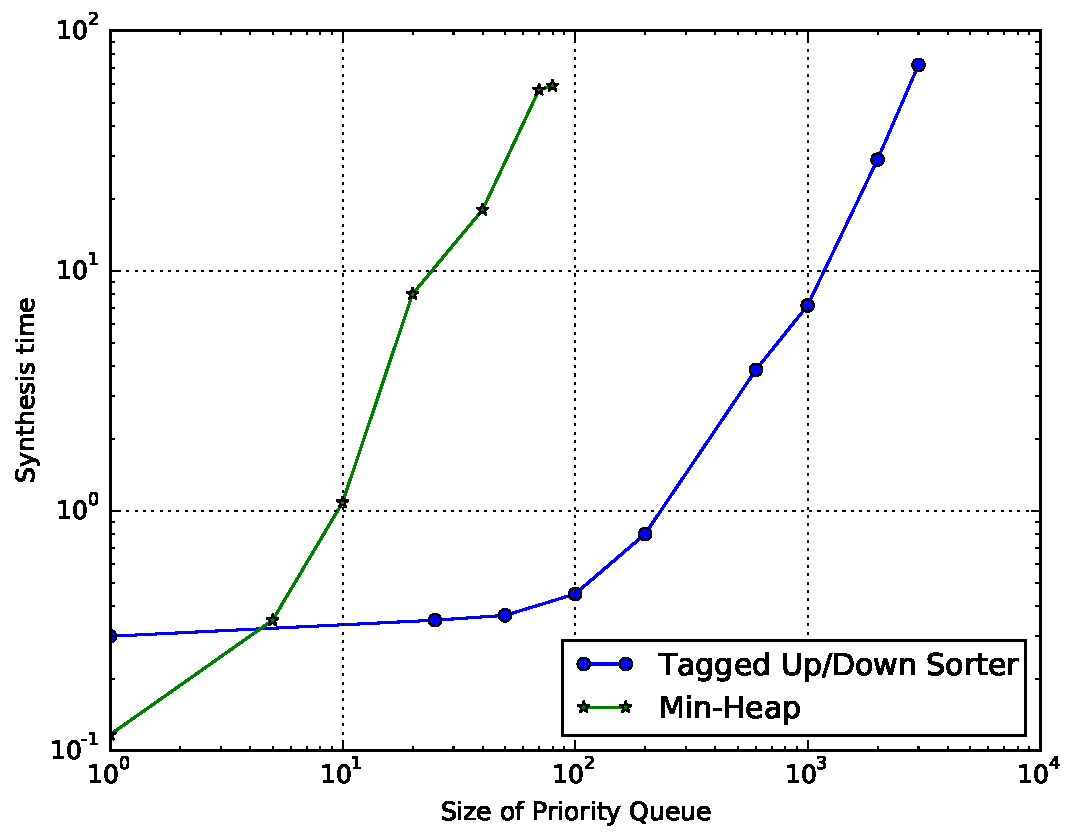
\includegraphics[width=\columnwidth]{data/synthesis_times.pdf}
	\caption{Synthesis Times}
	\label{fig:synth_times}
\end{figure}

In addition to these utilization numbers, I also present a plot of the time required for synthesis of each of the queue sizes to complete for the min-heap and the tagged up/down sorter for each queue size in Figure \ref{fig:synth_times}. From this plot, it can be seen that the time for synthesis increases quickly with the queue size, and is part of the reason for the limited performance results that I am able to present.

\subsection{Performance}
Performance is difficult to compare, since both of the published state-of-the-art implementations report performance in different ways. In addition, there is a lower bound of performance in that an operation cannot be performed faster than an FPGA clock cycle, since the queue is implemented with clock flip-flops. However, as the Tagged Up/Down sorter is implemented in Verilog to perform an enqueue or dequeue operation in a single clock cycle, it theoretically outperforms the state-of-the art solutions, as neither achieve this performance in both cases.

\begin{table}[t!]
	\centering
	\small
	\resizebox{\columnwidth}{!}{
	\begin{tabular}{| c | c | c |}
		\hline
		Queue Implementation & Test Execution Time & Number of Operations \\ \hline
		Tagged Up/Down Sorter & 131,402 $\mu$s & 67,000 \\ \hline
	\end{tabular}
	}
	\caption{Performance Results}
	\label{tab:perf}
\end{table}




